\begin{figure}[htb]
\begin{subfigure}[t]{0.35\textwidth}
    \centering
    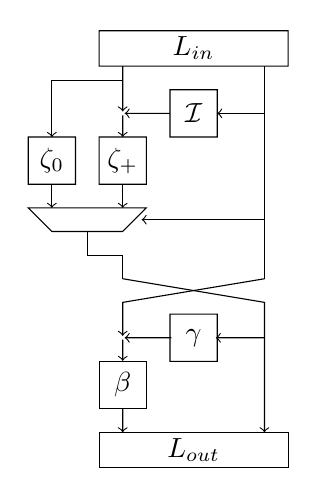
\begin{tikzpicture}[scale=0.6]
      % Drawing the S- and L- Boxes from bottom to top
      \draw (-2.00, -1.00) rectangle (+2.00, -0.25) node[pos=0.5]{$L_{out}$};
	  \draw (-2.00, +0.25) rectangle (-1.00, +1.25) node[pos=0.5,minimum size=0.6cm] (beta) {$\beta$};
      \draw
      (-0.50, +1.25) rectangle (+0.50, +2.25) node[pos=0.5,minimum size=0.55cm](gamma){$\gamma$}
      (-1.50, +1.75) node[inner sep=0] (mult_bottom) {$\fmult$}
      % Multiplexer
      (-1.50, +4.00) -- (-3.00, +4.00) -- (-3.50, +4.50) -- (-1.00, +4.50) -- (-1.50, +4.00)
      % Top part
      (-2.00, +5.00) rectangle (-1.00, +6.00) node[pos=0.5]{$\zeta_+$}
      (-3.50, +5.00) rectangle (-2.50, +6.00) node[pos=0.5]{$\zeta_{0}$}
      (-0.50, +6.00) rectangle (+0.50, +7.00) node[pos=0.5]{$\mathcal{I}$}
      (-1.50, +6.50) node[inner sep=0] (mult_top) {$\fmult$}
      (-2.00, +7.50) rectangle (+2.00, +8.25) node[pos=0.5]{$L_{in}$}
      ;
      % Arrows from bottom to top
%      \draw[->] (+1.50, +1.30) -- (+1.50, +0.75) ;
  %    \draw[->] (mult_bottom)  -- (+1.50, +2.20) ;
%      \draw[->] (+0.50, +3.00) -- (mult_bottom)  ;
      \draw (-2.25, +4.00) -- (-2.25, +3.50) -- (-1.50, +3.50) -- (-1.50, +3) ;
      \draw (+1.50, +7.50) -- (1.5, 3) ;
	
	% swap
	\draw[->] (1.5, 3) -- (-1.5, 2.5) -- (mult_bottom);
	\draw[->] (mult_bottom) -- (beta);
	\draw[->] (beta) -- (-1.5, -0.25);
	\draw[->] (-1.5, 3) -- (1.5, 2.5) -- (1.5, -0.25);
	\draw[<-] (mult_bottom) -- (gamma);
	\draw[<-] (gamma) -- (1.5, 1.75);


%      \draw[->] (-1.50, +3.00) -- (-0.50, +3.00) ;
      \draw[->] (+1.50, +4.25) -- (-1.10, +4.25) ;
      \draw[->] (-1.50, +5.00) -- (-1.50, +4.50) ;
      \draw[->] (-3.00, +5.00) -- (-3.00, +4.50) ;
      \draw[->] (mult_top)     -- (-1.50, +6.00) ;
      \draw[->] (-0.50, +6.50) -- (mult_top)     ;
      \draw[->] (+1.50, +6.50) -- (+0.50, +6.50) ;

      \draw[->] (-1.50, +7.50) -- (mult_top)     ;
      \draw[->] (-1.50, +7.20) -- (-3.00, +7.20) -- (-3.00, +6.00);
    \end{tikzpicture}
\end{subfigure}
\begin{subfigure}[t]{0.6\textwidth}
\vspace{-5cm} % hack..
\centering
      \renewcommand\arraystretch{1.3}
      \setlength{\tabcolsep}{2pt}
      \footnotesize
      \centering
      \begin{tabular}{l|rrrrrrrrrrrrrrrr}
 ~&~ $\hex{0}$ & $\hex{1}$ & $\hex{2}$ & $\hex{3}$ & $\hex{4}$ & $\hex{5}$ & $\hex{6}$ & $\hex{7}$ & $\hex{8}$ & $\hex{9}$ & $\hex{a}$ & $\hex{b}$ & $\hex{c}$ & $\hex{d}$ & $\hex{e}$ & $\hex{f}$\\
        \hline
        $\mathcal{I}$   ~&~ 0 & 1 & c & 8 & 6 & f & 4 & e & 3 & d & b & a & 2 & 9 & 7 & 5 \\
$\zeta_0$ ~&~ $\hex{2}$ & $\hex{5}$ & $\hex{3}$ & $\hex{b}$ & $\hex{6}$ & $\hex{9}$ & $\hex{e}$ & $\hex{a}$ & $\hex{0}$ & $\hex{4}$ & $\hex{f}$ & $\hex{1}$ & $\hex{8}$ & $\hex{d}$ & $\hex{c}$ & $\hex{7}$\\
$\zeta_+$ ~&~ $\hex{7}$ & $\hex{6}$ & $\hex{c}$ & $\hex{9}$ & $\hex{0}$ & $\hex{f}$ & $\hex{8}$ & $\hex{1}$ & $\hex{4}$ & $\hex{5}$ & $\hex{b}$ & $\hex{e}$ & $\hex{d}$ & $\hex{2}$ & $\hex{3}$ & $\hex{a}$\\
$\inv$ ~&~ $\hex{0}$ & $\hex{1}$ & $\hex{c}$ & $\hex{8}$ & $\hex{6}$ & $\hex{f}$ & $\hex{4}$ & $\hex{e}$ & $\hex{3}$ & $\hex{d}$ & $\hex{b}$ & $\hex{a}$ & $\hex{2}$ & $\hex{9}$ & $\hex{7}$ & $\hex{5}$\\
$\gamma$ ~&~ $\hex{1}$ & $\hex{d}$ & $\hex{1}$ & $\hex{6}$ & $\hex{5}$ & $\hex{3}$ & $\hex{a}$ & $\hex{5}$ & $\hex{e}$ & $\hex{7}$ & $\hex{9}$ & $\hex{6}$ & $\hex{8}$ & $\hex{7}$ & $\hex{e}$ & $\hex{1}$\\
$\beta$ ~&~ $\hex{0}$ & $\hex{e}$ & $\hex{b}$ & $\hex{4}$ & $\hex{2}$ & $\hex{3}$ & $\hex{f}$ & $\hex{8}$ & $\hex{a}$ & $\hex{7}$ & $\hex{1}$ & $\hex{9}$ & $\hex{5}$ & $\hex{c}$ & $\hex{6}$ & $\hex{d}$\\
      \end{tabular}
    %   \vspace{0.7cm}
    %   \TabDef{final}{The non-linear functions needed to compute $\pi$.}    
\end{subfigure}
\FigDef{final}{The decomposition of $\pi$. The multiplexer chooses its left input branch if the control branch is equal to zero, and its right input branch otherwise. $L_{in}$ and $L_{out}$ are given in Equation~\Ref{eq:lin}.}
\end{figure}
